\begin{figure}
    \begin{center}
    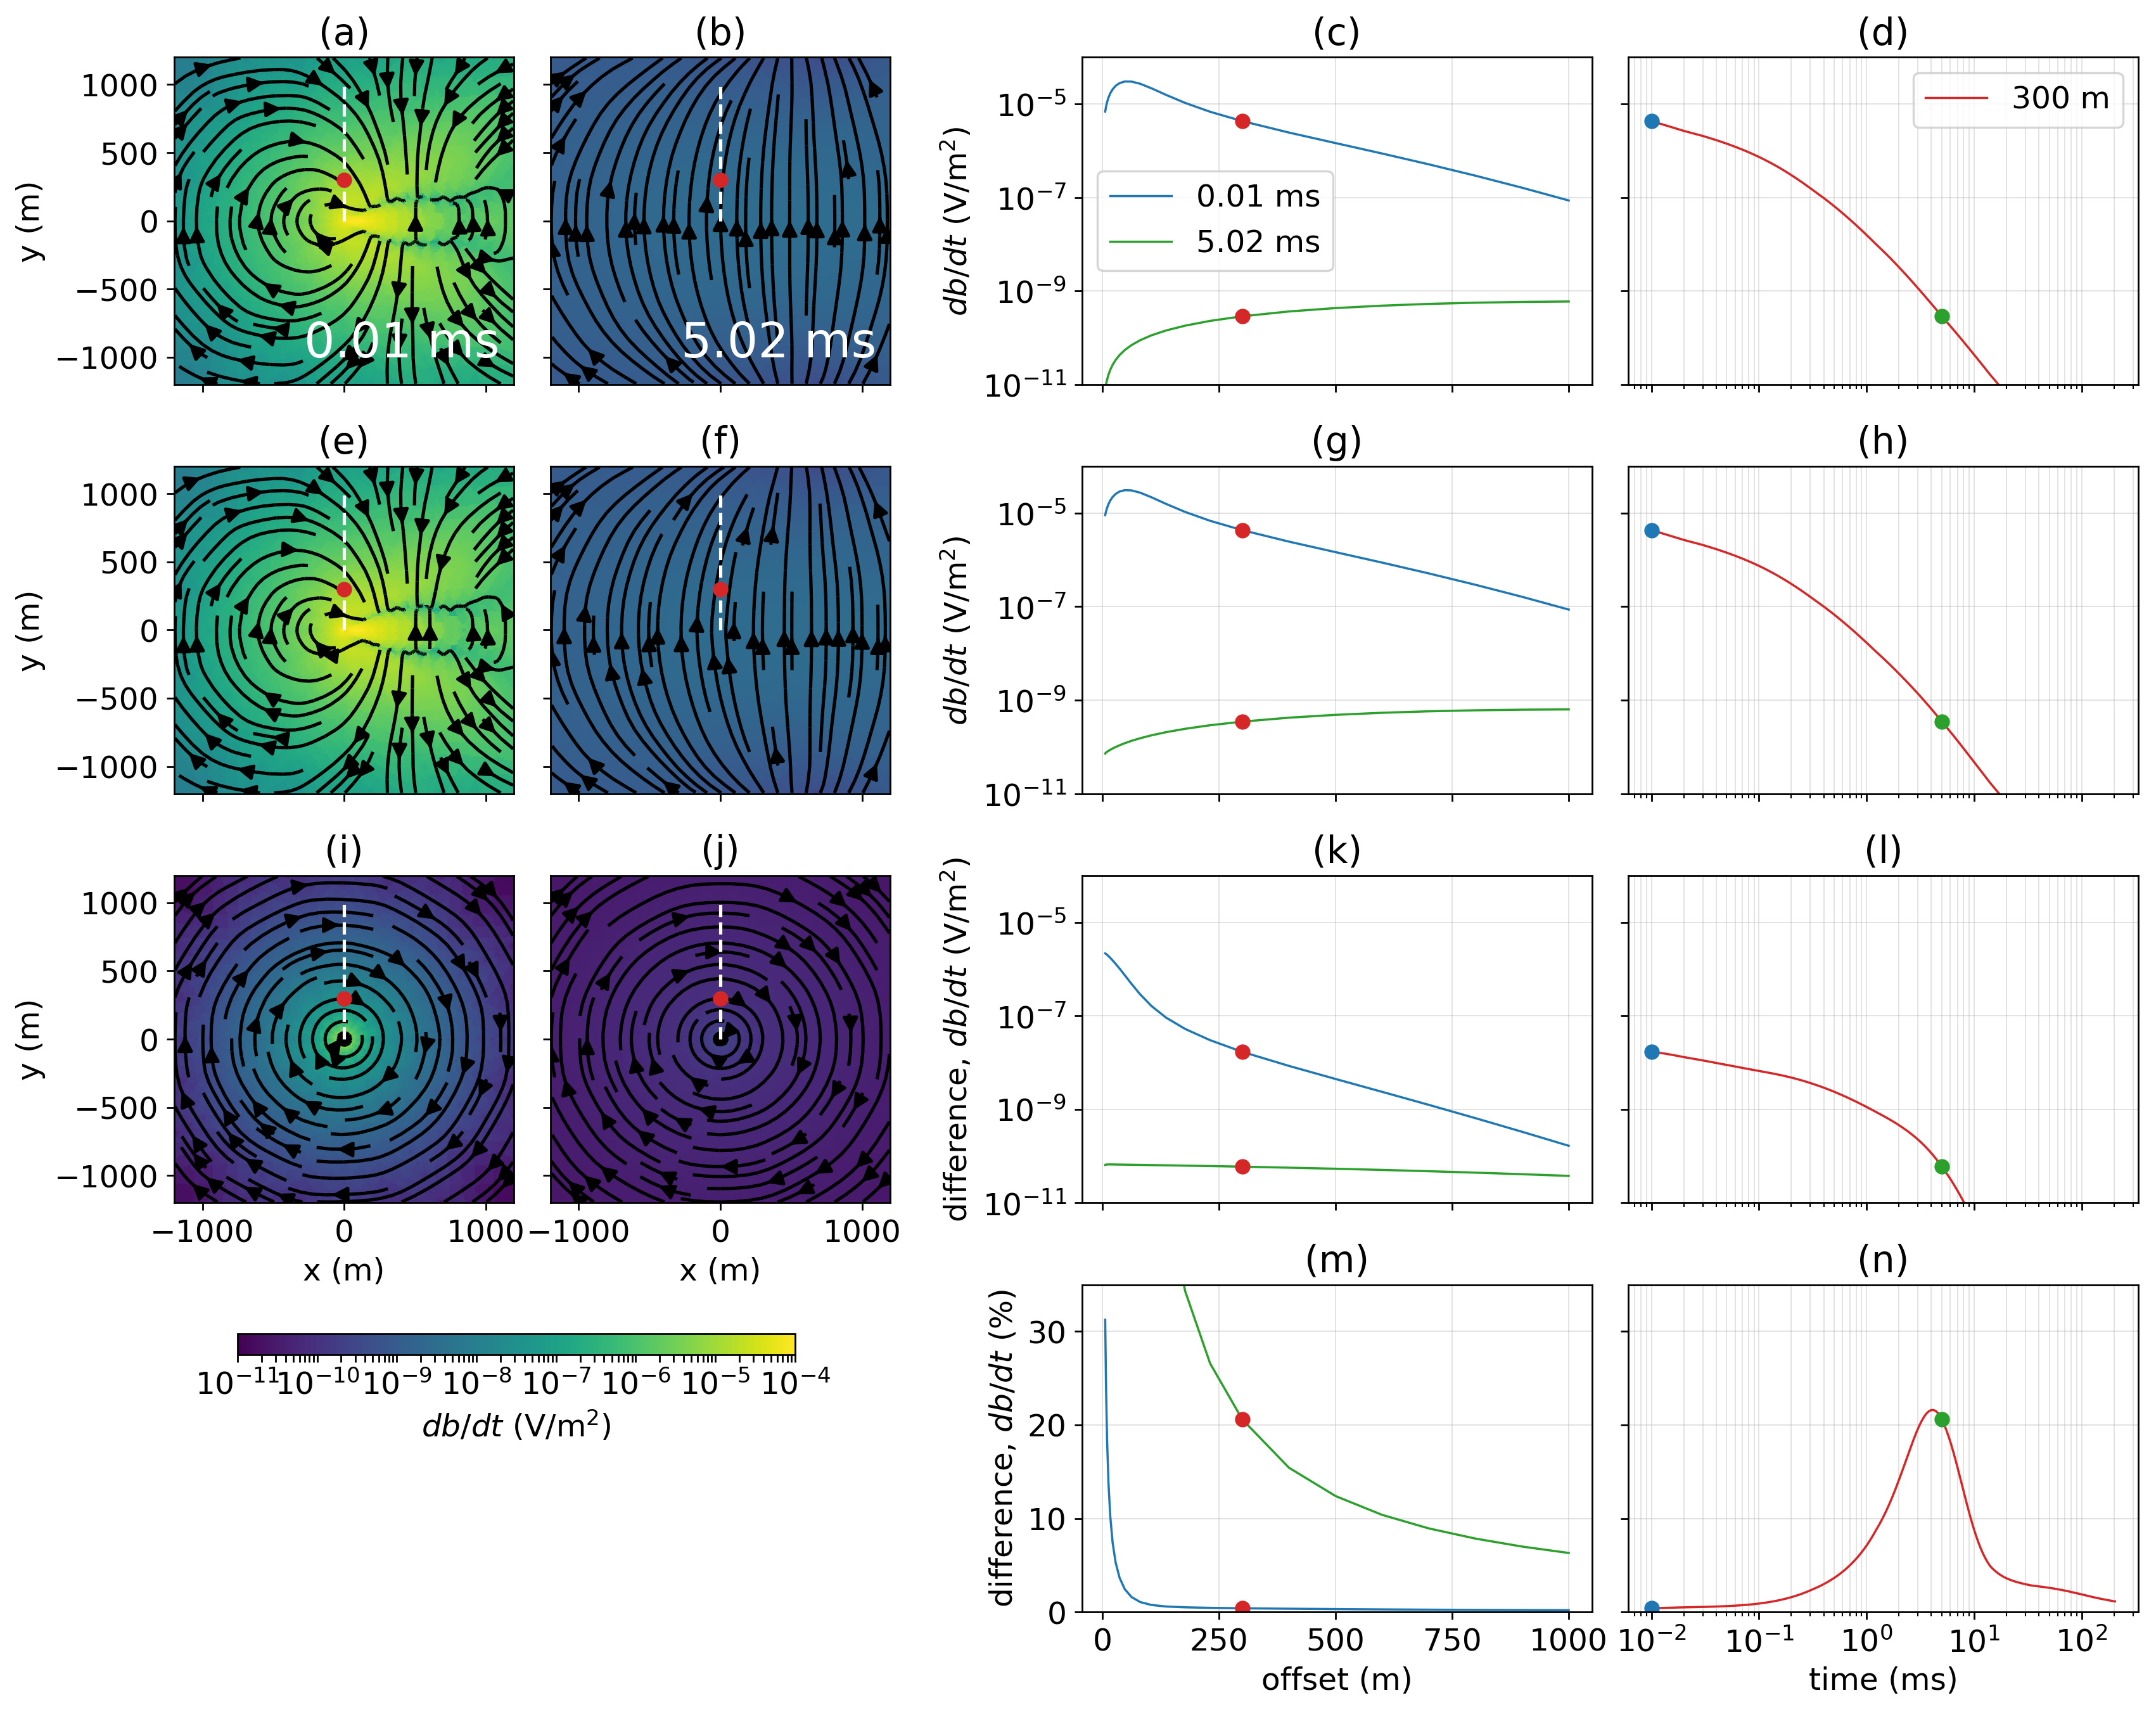
\includegraphics[width=\textwidth]{figures/em_casing/surface_dbdt_overview.png}
    \end{center}
\caption{
    Simulated $db/dt$ at (a) 0.01ms and (b) 5ms after shut-off for the halfspace model.
    (c) Tangential $db/dt$ measured along the white line in (a) and (b) at 0.01ms (blue) and 5ms (green).
    (d) Tangential $db/dt$ as a function of time at 300m along the survey line (shown in the red dot in (a)).
    Similar information is shown in (e), (f), (g) and (h) for the model with the conductive casing.
    The difference in the $db/dt$ data (casing minus halfspace) is shown in (i), (j), (k) and (l).
    The difference is also shown as a percentage of the halfspace solution at 0.01ms and 5ms in (m)
    and through time at 300m offset in (n).
}
\label{fig:surface_dbdt_overview}
\end{figure}



